\section{\label{I-A-1}Représenter le patrimoine aéronautique français : un musée aux collections uniques}

\subsection{La lente construction du \mae}

L'histoire du \acf{mae}\footnote{Voir la chronologie de l'histoire du musée en annexe \refinterne{Ax-A}.} est celle d'un projet persistant, sans cesse reporté et modifié, qui trouve ses racines dès la fin du XIXe siècle dans les aspirations d'associations ou de personnalités liées à l'aéronautique\footcite{terrierAeroportParisBourget2019}. Aujourd'hui encore, il ne cesse d'évoluer : l'année 2025 a ainsi vu, en plus de modernisations informatiques, l'inauguration d'un nouvel espace d'exposition permanente\footcite{museedelairetdelespaceHallNavigationAerienne2025} qui valorise la tour de contrôle de l'aéroport historique du Bourget. C'est en effet dans ces locaux que le musée s'est installé en 1973, après une longue période de recherches pour une implantation pérenne. Confronté aux aléas du XXe siècle, aux contraintes de conservation d'objets techniques et aux hésitations ministérielles, le projet d'installation doit sa concrétisation à l'engagement de militaires et de passionnés : ceux-ci ont su faire valoir le rôle du \mae comme vitrine d'un savoir-faire français pour obtenir son installation définitive.

La décision devient effective après la Première Guerre mondiale, premier conflit à exploiter l'importance stratégique de l'aviation. À l'initiative d'Albert Caquot, un conservatoire de l'aéronautique est confié au capitaine Hirschauer : quelques aéronefs trouvent refuge à Issy-les-Moulineaux, avant d'être déplacés à Chalais-Meudon à la suite d'une crue de la Seine. Le musée est officiellement inauguré le 23 novembre 1921 : l'institution naît, mais sans réel ancrage territorial. Pendant l'entre-deux-guerres, d'autres implantations sont tentées et notamment boulevard Victor à Paris. Ces locaux ouverts en 1936 ferment trois ans plus tard à l'aube de la Seconde Guerre mondiale. Bombardements et saisies allemandes interrompent son élan ; à la Libération, le musée réintègre Chalais-Meudon, mais demeure fermé au public durant plus de quinze ans.

S'ensuit une longue période d'incertitudes : entre 1952 et 1972, vingt-et-un sites sont envisagés\footcite{terrierAeroportParisBourget2019}. En 1961, le musée rouvre à Meudon, mais provisoirement. Le \enquote{Palais de l'Air} poursuit sa quête de locaux adaptés à la monumentalité de ses collections : en 1973, l'ancien aéroport du Bourget qui a été libéré au profit d'Orly est retenu comme implantation définitive.

Dès son ouverture, le musée affirme un lien fort avec l’État et l’industrie aéronautique : le prototype Concorde 001 lui est ainsi offert par l'état français à l'occasion de son inauguration. Cette position privilégiée lui permet de continuer sont développement, et à partir de cette date les collections sont progressivement transférées, Chalais-Meudon ferme en 1981, la direction rejoint le Bourget et de nouveaux halls sont ouverts au fil de l’extension du site. C'est avec l'ouverture d'un hall dédié à l'espace en 1983 que le musée prend son nom actuel : \acf{mae}.

Cette consolidation s’accompagne de son intégration à un réseau de musées techniques et de l'armée, et à d'importants chantiers de modernisation : un Planétarium est ouvert en 1985 et de nouvelles réserves permettant d'accueillir en hangars et en plein air les appareils des collections du musées sont installées à Dugny. L'informatisation des métiers du musée s'amorce dès les années 1990 avec la mise en place de \gls{micromusee} pour les collections, et du \ac{sigb} \gls{alexandrie}. En 2016, l’e-médiathèque est lancée pour gérer les fonds audiovisuels. La professionnalisation du musée est notamment marquée en 2002 par sa labellisation \enquote{Musée de France}. 

Ce mouvement de modernisation se poursuit aujourd’hui : les outils de gestion des collections du musées et de la bibliothèque ont été renouvelés définitivement en juillet 2025, de nouveaux espaces de conservation et d’exposition sont en projet, et l'intégration du musée au réseau du Grand Paris Express laisse espérer un surcroît de fréquentation.

Né tout d'abord de ses collections et non d'un site, le \mae, dédié à la mémoire du ciel, est aujourd'hui devenu indissociable de ses locaux emblématiques de l'aéronautique française pour devenir un musée incontournable.

\subsection{Une institution complexe qui fait référence}

C’est à partir des années 1980 que le musée se structure véritablement grâce à l’effet conjoint d’une reconnaissance de l’importance culturelle de l’aéronautique, d’un renouveau muséographique et de son inscription dans les réseaux nationaux. 

Son installation dans les locaux de l'ancien aéroport du Bourget incarne sa double fonction : conservatoire historique de l'aéronautique française, et vitrine stratégique d'un secteur en plein développement. Premier aérodrome civil parisien\footcite{terrierAeroportParisBourget2019}, ce lieu symbolique ancre en effet le musée dans la géographie et l’histoire de l’aviation française. Son lien avec le \ac{siae}, qu’il accueille tous les deux ans, renforce encore cette fonction de représentation.

La multiplicité des missions du \mae est parfaitement soulignée par Clémence Raynaud dans un article sur les collections iconographiques du \mae : tout d'abord dédié à la documentation de l'histoire et des techniques de l'aéronautique, le musée s'est développé \enquote{comme un établissement à vocation universelle embrassant de multiples aspects du fait aérien, que l’étiquette technique caractérise aujourd’hui d’une manière partielle\footcite{raynaudMuseeTechniqueDhistoire2018}.} Selon l'auteur, qui cite le \ac{psc} 2007, c'est autour des années 2010 que le musée s'affirme comme un \enquote{musée technique, d’histoire et de société}.

C'est là en effet l'un des grands défis auxquels il est confronté : le \mae possède des collections très riches et hétérogènes, sans équivalent national. On y trouve des aéronefs, moteurs, équipements techniques — objets exigeant des conditions de conservation particulières et une expertise rare. Cette spécificité impose des pratiques adaptées et des vocabulaires spécialisés. Mais le musée ne s’y limite pas : maquettes, estampes, objets d’art, uniformes, et, plus récemment, objets civils — vêtements, vaisselle, jouets — reflètent une évolution vers une muséographie anthropologique. Cette inflexion est incarnée notamment par la création d'un département des collections artistiques et anthropologiques, et la diversité des objets conservés se retrouve dans le schéma ci-dessous qui rassemble les différents noms de domaines des collections du musée.

\begin{figure}[htbp]
	\centering
	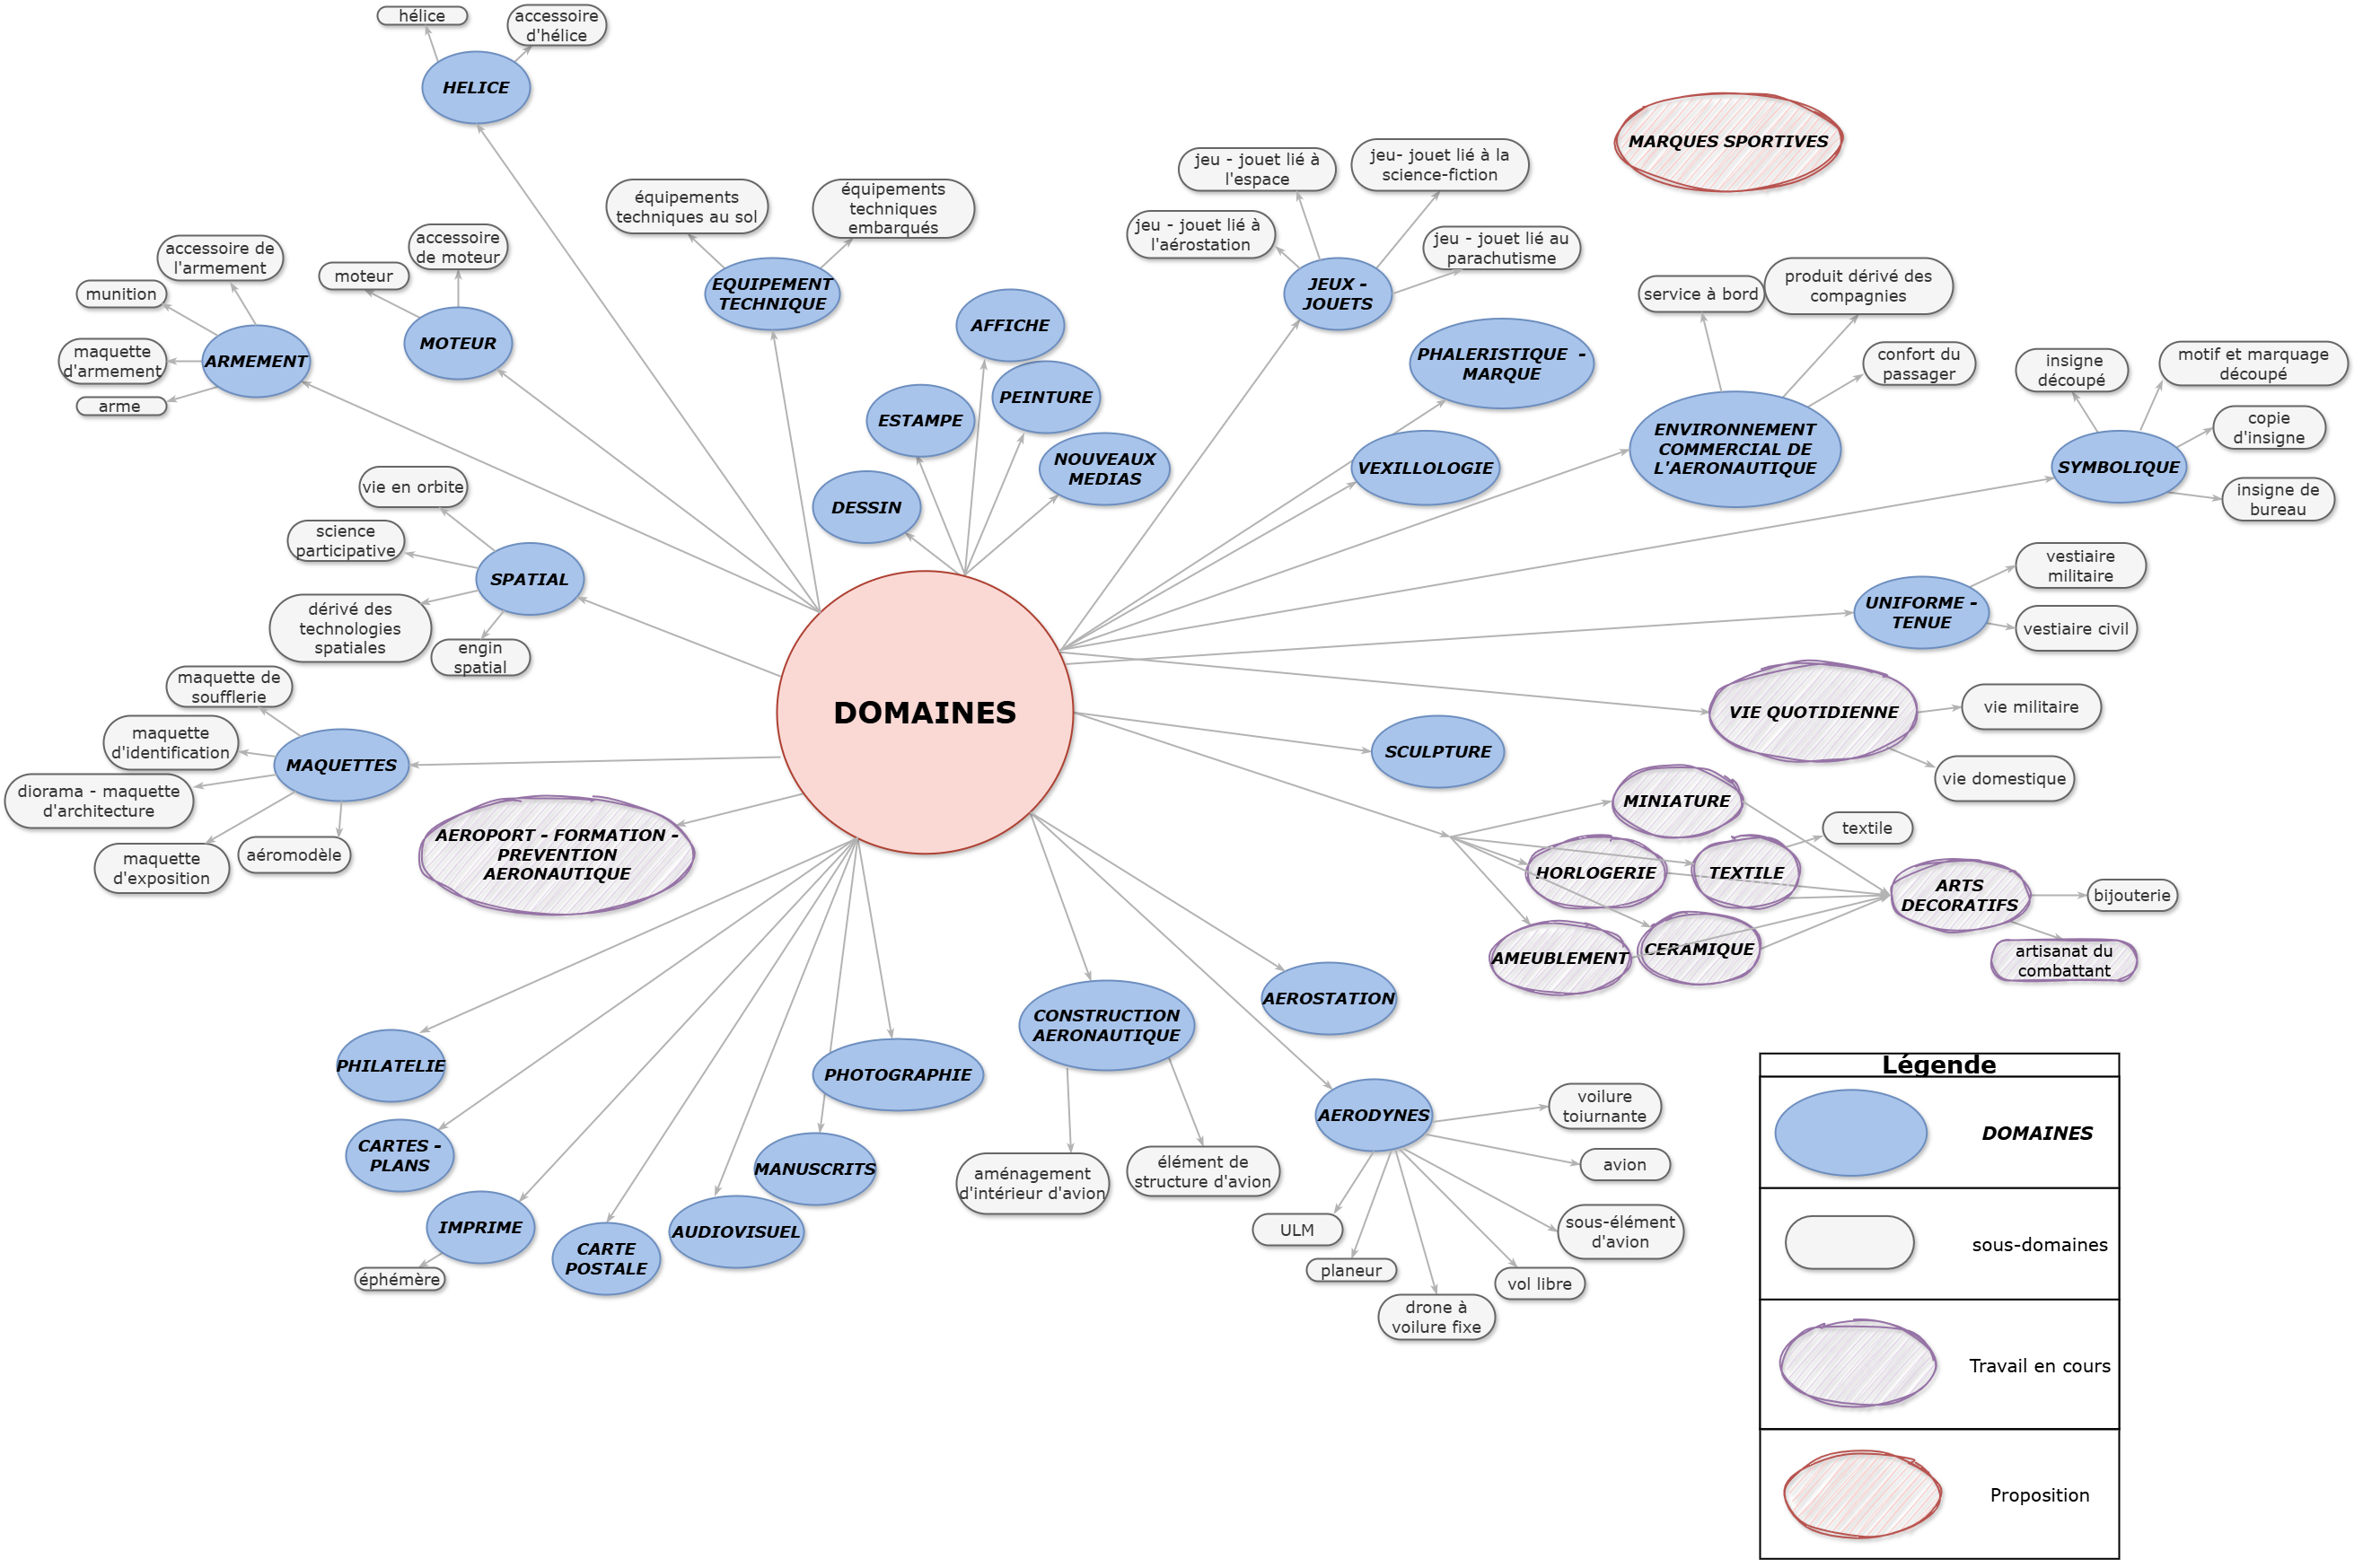
\includegraphics[width=\linewidth]{img/MODEL_domaines.png}
	\caption{Modélisation du thésaurus des domaines utilisés par le \mae}
	\label{fig:model_domaines}
\end{figure}

Le \mae incarne donc des défis propres aux musées techniques, bien différents de ceux des musées de beaux-arts, et imposent des compétences croisées à la fois techniques et muséales. Les jeunes chargés de collections sont ainsi souvent issus de formations spécialisés — comme les masters du Muséum d’histoire naturelle — et passent par des institutions techniques ou militaires, telles que le musée de la Marine, le musée de l’Armée ou le \ac{cnam}. Ceux-ci ont ainsi une expérience préalable avec ces objets singuliers, souvent massifs, complexes à restaurer et à exposer que conserve le musée.

Ces multiples défis sont rappelés par Agnès Mirambet-Paris et François Mirambet : diversité des matériaux, état de dégradation, inadéquation des environnements de conservation, échelle des objets, lourdeur des procédures, et besoin de ressources spécialisées sont au cœur des problèmes quotidiens de ces musées \footcite{mirambet-parisConservationrestaurationPatrimoineTechnique2011}. Ils insistent sur la nécessité du dialogue entre techniciens et restaurateurs :
\begin{quote}
	\og C’est bien par le partage de compétences techniques acquises dans le domaine industriel et celles obtenues dans les écoles de formation à la restauration que pourront se développer pleinement des travaux de restauration\footcite{mirambet-parisConservationrestaurationPatrimoineTechnique2011}.\fg
\end{quote}

Le \mae incarne cette articulation entre expertise technique et exigence muséale. Ses pièces emblématiques — comme le Concorde 001 ou le scaphandre de Jean-Loup Chrétien\footcite{champenoisTresorsMuseeLair2013} — en font une institution unique, au croisement des enjeux de représentation nationale, de préservation patrimoniale et d’innovation culturelle.
